\chapter{Financialization} \label{chapter-financialization}
\epigraph{Financialization  occurs when housing is treated as a commodity—a vehicle for wealth and investment—rather than a social good.}{Special UN Rapporteur on the right to adequate housing, Leilani Farha}


%https://www.ohchr.org/en/special-procedures/sr-housing/financialization-housing
%https://www.tni.org/en/publication/financialisation-a-primer#Q5
% This includes the housing market. By 2022 
% Financialization has become a major theme in Canadian discussions of what is increasingly seen as ..
Canada is experiencing what's increasingly seen as a national housing crisis. The Ontario Housing Affordability Task Force reported that ``This has home ownership beyond the reach of most first-time buyers across the province, ... Housing has become too expensive for rental units and ..  in rural communities and small towns. The system is not working as it should.''

Aled ab Iorwerth, Deputy Chief Economist at CMHC argued
\begin{quotation}
     “… Canada’s approach to housing supply needs to be rethought and done differently. There must be a drastic transformation of the housing sector, including government policies and processes, and an ‘all-hands-on-deck’ approach to increasing the supply of housing to meet demand.”\cite{CanadaHousingSupply2022}
\end{quotation}
% TODO: NEED A FINANCIALIZATION IN CANADIAN HOUSING QUOTE 

Arguably financialization, %the increasing share of housing owned by investors, 
is playing an important role in this crisis. The term financialization has different meanings at different levels of analysis. In finance, it is a term for the process of developing the legal instruments that facilitate financial transaction. At the microeconomic level, it is a collective noun for the growth in the number of individual transactions that create or transfer financial assets. At a macro level it refers to the effect on the system itself of the new instruments and the increase in the type of transaction that they make possible.
% The word ``financialization'' has several quite different meanings.  

This thesis is a study of financialization of the housing market. It is this third meaning, the system level effects of financialization, that is our focus. The following sections, we discuss financialization in the context of each of the three meanings above, financialization as financial instruments, an increasing share of control, and a system level set of shifts, and introduce the approach of this thesis. 

\section{Financial instruments} \label{section-financial-instruments}
One meaning of financialization is the development  
% To financialize anything is to create 
a \gls{financial instrument} that represents it, and can be bought and sold as an investment.
% the invention of the mechanisms of financialization.

There are numerous kinds of financial instruments. Examples of financialization outside the housing system include stocks and stock markets, within the housing system, mortgages, and more recently Real Estate Investment Trusts.

\subsubsection{Stocks and stock markets}
Financial instruments do not just occur in the housing system. 
For example the \gls{joint stock company}, the basis of the modern stock market and an important mechanism for channeling investment into productive activity,  is probably the most important financial instrument in the capitalist economy.  Stock markets are % generally described as 
a primary means of %efficiently
mobilizing long-term savings and investment for fixed capital formation \cite{azfarMarketMobilizedCapital2003}.  

Originally a tool to allow a group of investors to pool their money, take on large projects, and to share risks, the stocks themselves rapidly became objects of trade and speculation. Share prices on the stock market are not tightly tied to the productivity of the company they represent, %, illustrating how the financial instrument can diverge from the real asset. % makes it clear that the financial instrument is something different from the real asset. 
%Most stock transactions however are speculative in nature 
% Stock transactions can also be speculative in nature, however, 
and there is significant disagreement about the link between stock investment and investment in productive real assets \footnote{Mork et. al \cite{morckStockMarketInvestment1990} identify four theories that attempt to explain the correlation between stock returns and subsequent investment. \begin{quotation}The first says that the stock market is a passive predictor of future activity that managers do not rely on to make investment decisions. The second theory says that, in making investment decisions, managers rely on the stock market as a source of information, which may or may not be correct about future fundamentals. The third theory, which is perhaps the most common view of the stock markets influence, says that the stock market affects investment through its influence on the cost of funds and external financing. Finally, the fourth theory says that the stock market exerts pressure on investment quite aside from its informational and financing role, because managers have to cater to investors' opinions in order to protect their livelihood. For example, a low stock price may increase the probability of a takeover or a forced removal of top management. If the market is pessimistic about the firm's profitability, top management may be deterred from investing heavily by the prospect of further erosion in the stock price.\end{quotation} None of the point to a direct connection between stock market investment and real investment.}. 

Financial instruments can be combined and new types of instruments built on top of them. For example,
mutual funds, which pool more risky stocks, in an effort to offer more reliable returns, are a financial instrument built on top of the stock market.

\subsubsection{Mortgages}
An example of a foundational financial instrument that changed the structure of the housing market is the mortgage.  The mortgage demonstrates the two aspects of financial instruments. It is both a financial instrument that enables  purchase and a financial asset that can be bought and sold. 

Mortgages, for example, are a financial instrument that allows lenders to  participate in housing purchases in the present in exchange for a future flow of payments.  The mortgage does not create housing, but it enables the prospective buyer to become the nominal owner of an asset that produces a stream of benefits. The stream of benefits from secure housing near a source of income generally exceeds a buyer's current assets. The mortgage enables the transfer of ownership because it makes it possible to transfer the rights to a substantial fraction of the future income of the buyer to the mortgage holder who, in effect, is the owner until the terms of the mortgage are fulfilled.  If the mortgagee fails to make those payments the mortgage holder repossess the asset. The security provided by this instrument ``de-risks'' the transaction, making it safer and therefore easier to achieve the mutual benefits of the sale.

% Mortgages illustrate how not all financial instruments are instruments of financialization.  %***E MAYBE ADD IN WHAT SENSE... %like in the sense we mean, in the macro sense, in the technical sense of the word.. 
Mortgages are  financial instruments, but %another step is required to create a financialized  market in mortgages. 
the additional step of trading these mortgages on a market is required to create a financialized market. 
Originally mortgages were an arrangement between just the buyer and the seller, but in the 1870s in the USA, insurance companies stepped into these transactions, paying off the seller and then collecting the principle and interest payments on behalf of the bank's shareholders. This innovation was an example of financialization that made it possible for individual insurance companies to profit by providing money to buyers. When mortgage lending was regulated and insured  by the American government during and after the great depression it facilitated a massive increase in home ownership in the USA and contributed to the post-war construction boom and the suburbanization of American cities. The housing market was financialized by the market for insurance backed mortgages.

These mortgages were still agreements between individual lenders and buyers. When financial institutions, later,  developed markets that let them buy and sell bundles of mortgages among themselves, we say the mortgage market itself was financialized. There was then this further layer, a market for the promises to pay, in addition to the market for housing financed by % and the market for 
mortgage-type loans.

The transactions in this market, for promises to pay, do not directly affect the mortgage conditions or the home. They simply add a new product for investors or banks to buy and sell. This new market was thought to further reduce the risk for lenders, but between 2007 and 2010 in the USA the sub-prime mortgage crisis destabilized the financial institutions that were playing this new market. \footnote{Arguably, that crisis resulted from overselling risky and predatory mortgages by lenders with more money to lend than the market could absorb. Eager investors seeking higher or more secure returns were willing  to buy bundles of  mortgages that were in theory de-risked. Pooling uncorrelated individual risk, as the insurance industry does, produces lower overall risk. (The instruments that enabled the speculative bubble were mortgage-backed securities (MBSes) and collateralized debt obligations (CDOs).) Pooling does not reduce systemic risk, however. As it turned out, the mortgage default rate rose, lenders' liquidity fell, mortgage rates were pushed up, defaults increased, and the market for the new instruments collapsed, taking down major financial institutions, providing a cautionary tale about potential costs of financialization.} % While the details don't matter for this thesis, they provide a cautionary tale about the the potential costs of financialization.}.  

\subsubsection{Investment trusts}
An example of a financial instrument designed specifically to support rent extraction and which increases the degree of financialization of the housing supply is the Real Estate Investment Trust (\gls{REIT}).  A REIT is a company that owns, operates, or finances income-generating real estate and distribute the income to shareholders. While the company itself is an management system, the shares are are simply financial assets that are that are sold to individuals and organizations that want to share in real estate revenues and capital gains. There are other large owners of residential real estate such as life insurance companies and pension plans that behave similarly, but REITs are a relatively new financial instrument which is  expanding rapidly and attracting political attention for their effect on housing markets.  % REITs that develop new properties generally don't sell the properties they construct.

Developed in the USA  in 1960 (as an amendment to the Cigar Excise Tax Extension!) and in Canada in 1993 \cite{GET_REITsDevelopedDates}, REITs are similar to mutual funds in making it possible for an individual, often small investors to earn dividends from real estate investments without having to buy, manage, or finance any properties themselves. 

REITs have become increasingly popular in recent years.  An S\&P-Dow Jones research bulletin reported that over the  25 years to 2017, REITs outperformed stocks, bonds, and commodities \cite{GET-Dow-Jones-research-bulletin}. %***E COULD YOU SAY THE RELATIONSHIP IN A WAY THE CLARIFIES THE RELEVANCE OF THIS NEXT SENTENCE? % ***E I MEAN LIKE IS THIS A SIDE EFFECT. IT FEEL LIKES THIS IS A BIT OF A THROWAWAY STATEMENT THAT MIGHT HAVE MORE TO IT? 
Because they have outperformed competing investments they have attracted  capital from other uses, particularly during the recent period of low interest rates.\footnote{There are questions about preferential tax treatment, and whether some REITs are really just inappropriately sheltered real-estate corporations. } For the purpose of this thesis, REITs are simply one of the mechanisms for the financialization of housing.

\section{Financial transactions and share of ownership}

Financialization is not just the development of instruments. 
% The word also refers the the take up, the adoption as well. % It is the innovation not just the invention.
% it is also the increasingly control derived from the development of these kinds of mechanism. 
At the microeconomic level,  a second meaning of financialization is as a collective noun for the growth in the number of individual transactions that create or transfer financial assets. 
% We say that financialization is occurring if there is an increase the stock of financial assets associated with a stock of real assets. The development of new instruments facilitates this process, however the development of instruments in itself is not financializaiton, it requires that there is a market. 
% We have called attention in this section to the development  several important financial instruments -- mortgages, stocks, and REITs --  with the intention of  disentangling the concept of financial instruments from the term ``financialization''. 
% However, financialization is not a new concern.
More generally, financialization also describes the development of financial capitalism during the period from 1970 to present, in which debt-to-equity ratios increased and financial services accounted for an increasing share of national income relative to other sectors. % CIT

While there is no clear point in time when global financialization began, Thomson and Dutta,  \cite{thomsonFinancialisationPrimer2018}, suggest that 15 August 1971, when President Richard Nixon announced that the United States would unpeg the dollar from gold, marks a break point. The accelerated growth in global liquidity and prompted a surge of financial liberalisation and deregulation and undermined the Bretton Woods System.  Synthetic derivatives were created soon after: The Chicago Mercantile Exchange launched futures contracts written on financial instruments the following year and the Chicago Board of Trade introduced the first interest rate future contracts three years later. Arbitrage, options trading, and various other activities grew exponentially. By 2011, the over-the-counter (OTC) and exchange-traded derivatives market amounted to almost \$800 trillion.  %**MAKE MORE CLER WHAT THESE THINGS MEAN. 

By this definition, a subtantial and rising share of the economy and the housing system is financialized. 
In 2013, Tomaskovic-Devey and Lin wrote that ``The U.S. is now a financialized economy, where the financial sector and its priorities have become increasingly dominant in all aspects of the economy''\cite{tomaskovic-deveyFinancializationCausesInequality2013}. 

ADD FACTS 70\% of new units in Ontario/Waterloo bought by investors.
Sixty-six percent of Canadian homes are owner-occupied and about a third of the value of the homes is held as mortgages. Approximately two-thirds of the net land rents associated with housing, therefore, accrue to owner-occupiers \cite{nemtinFinancializationHousingSocial2021} CHECK. %{\color {red}CHECK THESE NUMBERS AND IF THEY CITE A BETTER SOURCE WE SHOULD GET} 


\section{Systems change}
Financialiation is % described as 
``a process whereby financial markets, financial institutions, and financial elites gain greater influence over economic policy and economic outcomes. Financialization transforms the functioning of economic systems at both the macro and micro levels'' \cite{palleyFinancializationWhatIt2007}. 
The third meaning of the word financialization refers to these effects of financialization at a systems level. 
% This process of financialization also has profound impact at systems level. 
% And the word financialization, at the macro level, refers to this set of impacts.

Figure~\ref{fig:Financialization-expansion} illustrates financialization of the housing market as a flow of money into the housing market, expanding financial ownership and tenancy while reducing the share of owner-occupied housing. Its goal is the capture of spatial rents, which we will show has implications for both the productivity and the class structure of the city. 
In the urban context financialization is fundamentally rent seeking, and we argue it can have a profound impact on the system, including effects on both distribution and productivity.  

\begin{figure}
\begin{center}
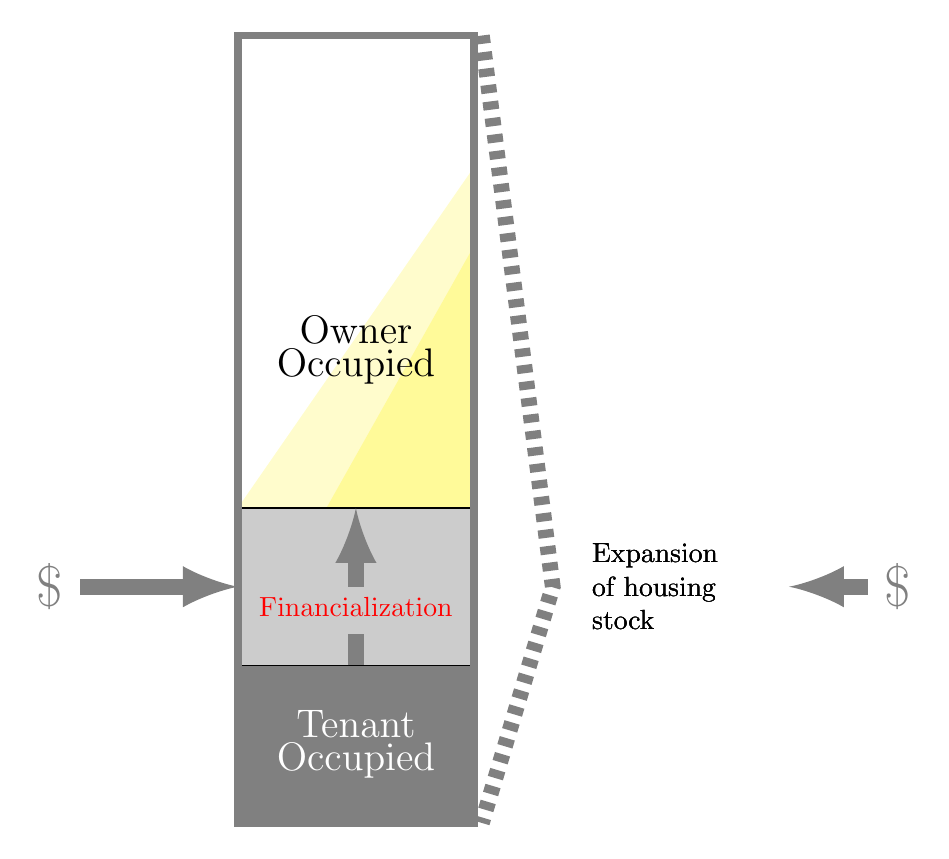
\begin{tikzpicture}{scale=.5}
\draw [fill=yellow!20] (0,4)--(3,4)--(3,8.33); --cycle;% MORTGAGE %Calculation. 80\%owner, so  8 above the tenant line. 2/3*8=5.333. 5.333+2=

\draw [fill=yellow!40] (0,2)--(3,2)--(3,7.33); --cycle;% MORTGAGE %Calculation. 80\%owner, so  8 above the tenant line. 2/3*8=5.333. 5.333+2=
\draw [fill=gray!40,opacity=1] (0,0) rectangle (3,4); %fiancialization   
\draw [fill=gray] (0,0) rectangle (3,2); %TENANT

\draw[line width= 1mm, black!50] (0,0) rectangle (3,10);

\node at (1.5,6)
    [text width=2.4cm, align=center]
    {\baselineskip=20pt\Large Owner Occupied};
%\node at (2,3.3) [text width=2.4cm]  {\baselineskip=20pt Mortgaged};
\node at (1.5,1)
    [text width=2.4cm, align=center, white]
    {\baselineskip=20pt\Large Tenant Occupied};

%\draw [gray,line width=2mm](1.5,2)--(1.5,2.4) node[above, red]{Financialization}; 
\draw [gray,line width=2mm](1.5,2)--(1.5,2.4) node[above, red]{Financialization}; 
\draw [gray,-latex, line width=2mm](1.5,3)--(1.5,4);
%\draw [gray,line width=2mm,-latex](3,3)--(4,3);
\node at (5.5,3)[text width=2cm]{Expansion of housing stock}; 
\draw [gray, dashed,line width=2mm,](3.1,10)--(4,3)--(3.1,0);

\draw [gray,line width=2mm,-latex](-2,3)node[left]{\huge$\$$}--(0,3); \node at (5.5,3)[text width=2cm]{Expansion of housing stock}; 

\draw [gray,line width=2mm,-latex](8,3)node[right]{\huge$\$$}--(7,3); 
\node at (5.5,3)[text width=2cm]{Expansion of housing stock}; 
\end{tikzpicture}
\end{center}
 \caption{Financialization vs expansion of the housing stock }
\label{fig:Financialization-expansion}
\end{figure}

 % THOUGHT TO LOWER RISK  %DID THE CRISIS SHOW IT DIDN'T?

The instruments and share are not neutral tools. They have the potential to have a profound effect at the level of the system.

Mortgages can influence the system. 
When we consider urban housing, it is the right to future income generated by capital, labour, and the city itself through the agglomeration effects that drive productivity. It is an instrument that indirectly captures a share of the urban rents. As productivity rises, wages rise, rents rise, property prices rise and mortgages rise. 

REITS  are not simply a neutral tool for saving however. According to a paper \cite{wangAnalyzeImpactREITs2021} on REITS in the Irish housing market, ``REIT successfully reconnected the international financial market and the Irish real estate market.'' In other words, in Ireland, REITS have made it easier for international capital to buy Irish land. The entry of outside and footloose capital has had an effect on the resident population:  ``the large-scale acquisition of Irish real estate by REITs and other real estate buyers has also caused some new problems. First, the active management of assets by REITs and other investors has led to a rapid increase in rents''.\footnote{In  IMF working paper ``Capital Account Liberalization and Inequality'' \cite{furceriCapitalAccountLiberalization2015}  Furceri and Loungani reported that that for 149 countries from 1970 to 2010, ``after countries take steps to open their capital account, an increase in inequality in incomes within countries follows'' . The observation is consistent with our argument  that domestic rent-seeking in housing markets will increase inequality.}   

There is evidence that REITs affect real estate markets in other ways. Bat et all  \cite{batRolePublicREITs2022} reprot that  ``they are actually financial actors that aggressively buy up property assets and manage them to extract wealth at taxpayers’ expense. '' and ``they have expanded the pool of capital available for transactions that monetize real property and turn it into tradable assets – financial widgets with little or no connection to the real purpose of the productive enterprises that occupy the properties they own.''




There are different kinds of systemic effects of this kind of increasing control and coupling 
SYSTEMS DIAGRAMS
e.g.
The rising share- 
rising- actually has control, they have a political interest, become coupled, too big to fail.








\subsection{Systems design engineering and the systems level effects of financialization}
Appropriate for systems design engineering
- engineering is science to responsibility.


\section{Summary} %: Financialization in a modern urban theory of rent}
This chapter has discussed the theory of financialization.
Financialization, in our analysis, is the increasing control of the stock of urban land and housing by investors in order to capture the scarcity rent generated by the people of the city, and the system level effects of that increasing control.  The rest of the dissertation is an exploration of the systemic effects of financialization. 

% Financialization of the housing market is about
Financialization is about capturing the surplus in an urban economy so we next go to the theory of rent which is an theory accounting for distribution of surplus. 





